\documentclass[11pt]{article}
\usepackage[margin=1in]{geometry}
\usepackage{graphicx}
\usepackage{booktabs}
\usepackage{amsmath,amssymb}
\usepackage{microtype}
\usepackage{hyperref}
\usepackage{xcolor}
\usepackage{enumitem}
\usepackage[T1]{fontenc}
\usepackage[utf8]{inputenc}
\usepackage{float}

\graphicspath{{../results/figures/}}

\definecolor{note}{RGB}{60,80,140}
\newcommand{\note}[1]{{\color{note}\textit{#1}}}
\newcommand{\honest}[1]{\textcolor{red!70!black}{\textbf{Honesty note:} #1}}

\title{An Explainer:\\
Tracing Alveolar Cell Failure in Lethal COVID-19\\
with Single-Cell Trajectories and Ablation Tests}
\author{A guide for computational biologists, computer scientists, and biologists}
\date{\today}

\begin{document}
\maketitle

\begin{abstract}
\noindent This explainer walks through a class-project analysis of the Columbia/NYP COVID-19 Lung Atlas (SCP1219) end-to-end: why the biology matters, how the data were generated and prepared, what each computational step actually computes, how to read the plots and tables, what the ten ablations were designed to falsify, and --- crucially --- what the data support and what they do \emph{not}. Results are reported without overstatement: of three pre-registered criteria for ``epithelial robustness collapse,'' two were supported and one was not.
\end{abstract}

\tableofcontents
\bigskip

\section{The biology, in plain terms}

\subsection{What is the alveolar epithelium?}

Deep in the lung, roughly 480 million tiny air sacs (\emph{alveoli}) are where you actually exchange O\textsubscript{2} and CO\textsubscript{2} with your blood. The wall of each alveolus is lined by a two-cell epithelium:

\begin{description}[style=nextline]
\item[AT1 (alveolar type I) cells] Extraordinarily flat; they cover about 95\% of the alveolar surface. They are the \emph{gas-exchange barrier}.
\item[AT2 (alveolar type II) cells] Cuboidal; they secrete \emph{surfactant} (the lipid-protein film that keeps alveoli from collapsing at the end of exhalation) and act as the local \emph{stem cells}: when AT1 cells are destroyed, AT2 cells divide and differentiate into new AT1 cells through a transitional state marked by the genes \textbf{KRT8}, \textbf{CLDN4}, and \textbf{SFN}.
\end{description}

\subsection{What goes wrong in lethal COVID-19?}

SARS-CoV-2 enters AT2 cells via the ACE2 receptor. The virus is infecting the very cells that the lung depends on both for surfactant and for regeneration. On top of that, the immune response itself damages the epithelium (inflammatory ``collateral damage''). Autopsy studies describe diffuse alveolar damage: AT1 cells missing, edema, and abnormal cells that are neither cleanly AT1 nor cleanly AT2 --- apparently caught mid-repair. The core question of this project: does the alveolar epithelium fail as a \emph{coherent block} (all the cells move to a new damaged state), or does it fail as a \emph{graded, continuous process} (cells fan out along a spectrum of states)?

\section{The data}

\subsection{Where they came from}

We used a publicly available dataset: the \emph{Columbia/NYP COVID-19 Lung Atlas} (Broad Single Cell Portal accession SCP1219; Melms et al., \textit{Nature}, 2021). The dataset was generated from post-mortem lung tissue from 20 COVID-19 donors and 7 healthy organ donors. Nuclei were extracted from frozen tissue and sequenced with single-nucleus RNA-seq (snRNA-seq), giving 116{,}313 nuclei $\times\sim$30{,}000 genes.

\note{Why single-\emph{nucleus} rather than single-\emph{cell}? In post-mortem tissue, whole cells don't survive freeze/thaw well, but nuclei do. The trade-off is that snRNA-seq captures mostly unspliced (nascent) transcripts and biases composition differently than scRNA-seq.}

\subsection{What we kept}

We retained only alveolar epithelial cells --- the ones whose biology the question is about --- by filtering on the atlas's own fine cell-type labels (\texttt{cell\_type\_fine} $\in$ \{\texttt{AT1}, \texttt{AT2}, \texttt{ECM-high epithelial}\}). That left \textbf{22{,}128 cells}: 9{,}608 AT1, 11{,}341 AT2, 1{,}179 ECM-high transitional (all 27 donors contributed).

\honest{Per-donor cell counts ranged from 62 to 2{,}850; 10 of 27 donors contributed fewer than 300 alveolar cells. We relied on leave-one-donor-out (Section~\ref{sec:ablations}, Ablation 7) to check that no single donor drove any finding.}

\section{The computational pipeline, step by step}

A high-level picture: take the cell-by-gene count matrix, clean it, reduce its dimensionality, lay out the cells in a ``landscape'' (the manifold), order the cells along that landscape by a pseudotime, score each cell for biologically curated gene programs, and then test where COVID-19 cells sit versus healthy cells.

\subsection{Normalization and feature selection}

\begin{enumerate}
\item \textbf{Total-count normalization}: divide each cell's counts by its total, then multiply by a fixed target (10{,}000). This removes the ``some cells are sequenced deeper than others'' artifact.
\item \textbf{log1p transformation}: $x \mapsto \log(1+x)$. This stabilizes variance so highly expressed genes don't dominate distance calculations.
\item \textbf{Highly-variable gene (HVG) selection}: keep the 3{,}000 genes whose expression varies the most across cells, using the Seurat v3 method (it fits the mean-variance relationship of raw counts and keeps the genes that deviate most upward).
\end{enumerate}

\note{For a computer scientist: this is a feature-selection step. We drop genes whose variance is ``explainable'' under a null mean-variance model. For a biologist: the idea is to keep the genes that carry biological signal (identity, stress response) and drop the many that are stably expressed or just noisy.}

\honest{One specific gene, \textbf{GPX1} (glutathione peroxidase 1), was absent from the HVG set. Because our downstream gene-program scoring operates on the full expression matrix, this mostly matters in a subtle way: other programs may have analogous silent dropouts that we did not exhaustively audit.}

\subsection{Dimensionality reduction}

\begin{enumerate}
\item \textbf{Scale}: z-score each gene (clipped at 10).
\item \textbf{PCA}: 50 principal components. Linear projection that preserves global structure and denoises.
\item \textbf{Batch correction (attempted)}: we configured Harmony (harmonypy 0.2.0) with donor as batch key. \emph{It failed at runtime.} The library returned a 1-D array of shape (50,) where a (22128, 50) matrix was expected. The pipeline detected this and fell back to uncorrected PCA. Ablation 3 was intended to compare ``corrected vs.\ uncorrected,'' but both branches ended up being uncorrected.
\item \textbf{$k$-NN graph}: for each cell, find its 15 nearest neighbors in PCA space. Edges encode transcriptomic similarity.
\item \textbf{UMAP} (2D): a non-linear, neighborhood-preserving embedding for visualization. Never trust distances on UMAP for statistical claims; use it to \emph{see} structure.
\item \textbf{Diffusion map} (15 components): a nonlinear embedding from the $k$-NN graph's transition matrix. This is what we actually use for trajectory inference.
\end{enumerate}

\subsection{Pseudotime}

\textbf{Diffusion pseudotime (DPT)} is a scalar per cell. Conceptually: pick a starting cell (\emph{root}), then for every other cell compute a distance along the diffusion-map manifold. That distance is the pseudotime.

\note{It is \textbf{not} real elapsed time. It is an ordering along the manifold, interpretable as ``how far from the root state is this cell?''}

The root we used: the cell closest to the centroid of healthy AT2 cells in diffusion-map space. Rationale: healthy AT2 is the canonical starting point of alveolar self-repair (AT2 $\rightarrow$ transitional $\rightarrow$ AT1). We tested this root-choice explicitly with Ablation 5 (four alternative roots; see Section~\ref{sec:ablations}).

\subsection{Gene-program scoring}

A \emph{gene program} is a biologist-curated list of genes associated with one process. We used 8 programs:

\begin{itemize}[leftmargin=1em,nosep]
\item AT2 identity (SFTPC, SFTPA1/2, \dots)
\item AT1 identity (AGER, HOPX, PDPN, \dots)
\item Interferon response (ISG15, IFIT1, MX1, STAT1, \dots)
\item NF-$\kappa$B inflammatory (NFKB1, TNF, IL6, IL1B, \dots)
\item Oxidative stress (SOD1/2, CAT, HMOX1, NRF2/NFE2L2, \dots)
\item AT2$\rightarrow$AT1 differentiation (KRT8, CLDN4, SFN, LGALS3, \dots)
\item Apoptosis (BAX, BAK1, CASP3/7/9, \dots)
\item Senescence (CDKN1A/p21, CDKN2A/p16, IL6, IGFBP7, \dots)
\end{itemize}

Scoring uses Scanpy's \texttt{score\_genes}: the mean expression of the program's genes minus the mean of a random background of similarly-expressed genes. \alert{The scale of one program's score is not directly comparable with another program's.}

\section{How we defined the question we wanted to answer}

We pre-registered three operational criteria for ``epithelial robustness collapse,'' each a statistical test:

\begin{enumerate}
\item \textbf{Centroid displacement}: one-sided Mann--Whitney $U$ on per-cell Euclidean distance to the healthy-condition centroid in PCA-50. Alternative: COVID-19 cells are \emph{farther} than healthy cells from the healthy centroid.
\item \textbf{Within-group dispersion}: Levene's test comparing the distributions of distance-to-own-centroid between conditions. Larger variance under COVID-19 would mean cells spread out more.
\item \textbf{Pseudotime enrichment}: median pseudotime difference (COVID $-$ Healthy), with a 1{,}000-iteration permutation null (labels shuffled).
\end{enumerate}

Composite: \emph{strong} if all 3 significant, \emph{moderate} if 2, \emph{weak} if 1, \emph{not supported} if 0.

\section{Results, carefully}

\subsection{Finding 1: a real but modest pseudotime shift}

Control median pseudotime 0.063; COVID median 0.111; observed difference $+0.0483$ on a $[0,1]$ normalized axis. Under 1{,}000 label permutations the null was tightly centered at zero (mean $6\times 10^{-5}$, std $1.2\times 10^{-3}$), and the observed value was never exceeded $\Rightarrow$ empirical $p = 0.000999$.

\begin{figure}[H]
\centering
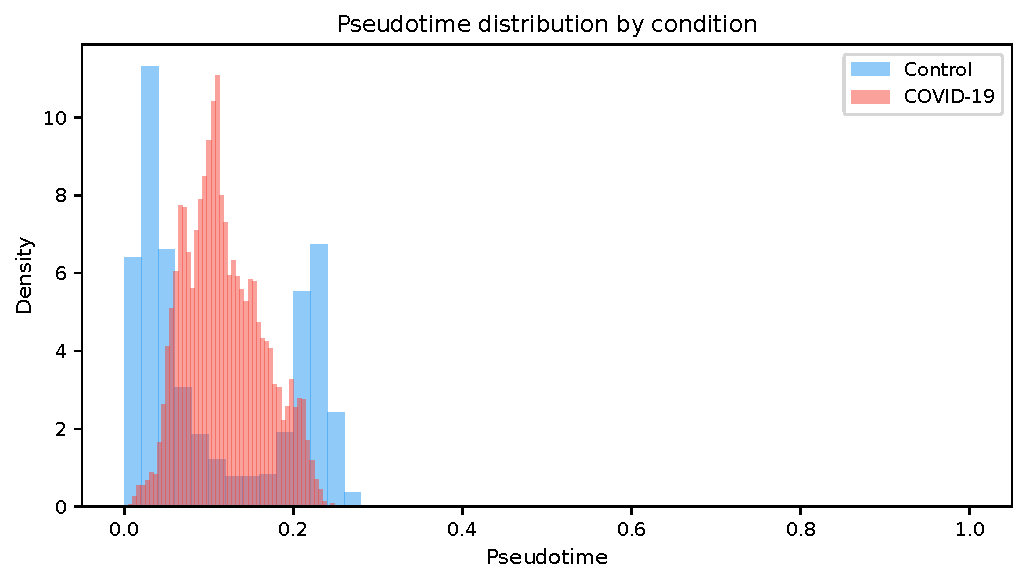
\includegraphics[width=0.7\linewidth]{fig4_pseudotime_density.pdf}
\caption{Pseudotime density by condition. COVID-19 distribution shifted toward higher pseudotime.}
\end{figure}

\honest{Magnitude is modest (4.8\% of the normalized axis). Pseudotime is unit-less; this is not a ``4.8\% worse'' claim --- it's an ordering shift.}

\subsection{Finding 2: centroid displacement \textbf{failed}}

One-sided Mann--Whitney $U$ in PCA-50 (COVID $>$ Healthy): $U = 5.21\times 10^7$; $p = 1.0$. Medians go the ``wrong'' way: COVID 10.68, Healthy 11.56. Rank-biserial $r = 0.14$.

\begin{figure}[H]
\centering
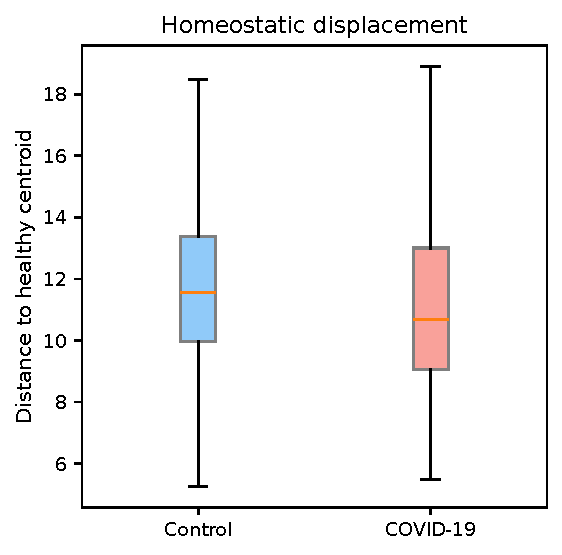
\includegraphics[width=0.7\linewidth]{fig5b_displacement.pdf}
\caption{Distance-to-healthy-centroid distributions. The distributions largely overlap; mean and median do not distinguish conditions in the pre-specified direction.}
\end{figure}

\honest{A pre-registered criterion was \textbf{not supported}. We don't bury this. It is the most important robustness-collapse test that did \emph{not} work as hypothesized, and it shapes the whole interpretation: COVID-19 cells do not uniformly move \emph{away} from the healthy centroid; some stay close, others go far, and the average is roughly unchanged.}

\subsection{Finding 3: dispersion \emph{did} succeed}

Variance of distance to own-condition centroid: COVID 33.28 vs.\ Healthy 14.58 (2.3$\times$). Levene statistic 276.5; $p < 10^{-30}$.

\note{This is exactly the pattern a centroid-displacement test would \emph{miss}: COVID-19 cells are not systematically shifted; they are systematically \emph{spread out}.}

\subsection{Finding 4: program ordering along pseudotime}

\begin{table}[H]\centering\small
\begin{tabular}{clrr}
\toprule
Rank & Program & Peak pseudotime & Peak score \\ \midrule
1 & AT2 identity & 0.015 & 0.75 \\
2 & AT1 identity & 0.266 & 1.25 \\
3 & Apoptosis & 0.591 & 0.17 \\
4 & AT2$\rightarrow$AT1 diff.\ & 0.744 & 0.57 \\
4 & NF-$\kappa$B & 0.744 & 0.18 \\
4 & Oxidative stress & 0.744 & 0.21 \\
7 & Interferon & 0.866 & 0.33 \\
8 & Senescence & 0.935 & 0.24 \\ \bottomrule
\end{tabular}
\end{table}

Homeostatic identity programs peak at low pseudotime; injury programs cluster in the upper half. \honest{This is \textbf{not} the cleaner hypothesized order (interferon first, apoptosis last). Apoptosis peaks \emph{before} interferon. Whether this is biology or an artifact of gene-list choice / score-genes normalization is exactly what Ablation 8 probes --- and it matters, because swapping curated lists for MSigDB hallmark sets \emph{inverts} the ordering ($\rho = -0.80$).}

\subsection{Finding 5: KRT8\textsuperscript{+} transitional population}

ECM-high / KRT8\textsuperscript{+}/CLDN4\textsuperscript{+} transitional cells were 3.1$\times$ enriched in COVID-19 (8.5\% vs.\ 2.7\%; $\chi^2$ $p < 10^{-30}$) and concentrated at intermediate pseudotime (mean 0.3--0.5). Their marker signature matches damage-associated transient progenitors described in mouse lung injury and IPF. Interpretation: a sub-population looks like cells that \emph{initiated} AT2$\rightarrow$AT1 repair but did not complete it. \honest{This is a snapshot correlation, not a lineage trace. We cannot prove any individual cell was mid-transition.}

\section{The ten ablations: what they were and what they showed}\label{sec:ablations}

Each ablation modifies one methodological choice and reruns the core analysis. An ablation ``passes'' if the three summary metrics retain the same sign/qualitative interpretation as the primary analysis.

\begin{description}[leftmargin=1.3em,style=nextline]
\item[1. AT2-only subset.] MPD $+0.133$ (larger!); program ordering $\rho = 0.33$ (weaker); displacement $r = -0.29$ (\emph{sign flip}). Non-displacement finding is stronger, not weaker, when restricted to AT2.
\item[2. Embedding variants (UMAP vs.\ diffmap-augmented).] Both identical to primary. Pseudotime shift does not depend on embedding choice.
\item[3. With vs.\ without batch correction.] Both branches identical to primary --- because Harmony failed and both fell back to uncorrected PCA. \honest{This ablation is effectively \emph{degenerate}: it does not test what it was designed to test.}
\item[4. Remove apoptosis genes before HVG selection.] MPD slightly up, ordering moderately degraded. Apoptosis genes weren't driving the shift.
\item[5. Four alternative pseudotime roots.] Shift magnitude varies ($-0.037$ to $+0.048$); ordering inverts under COVID-extreme root. Primary root gives the largest and most consistent signal. \alert{Pseudotime direction is root-dependent; declare your root.}
\item[6. Broader epithelial (alveolar + airway).] MPD collapses to $-0.008$. \textbf{Adding airway cells abolishes the pseudotime shift.} The trajectory is specifically alveolar. Pooling compartments dilutes the signal.
\item[7. Leave-one-donor-out (27 iters).] All 27 preserve the direction; range 0.028--0.202; bulk 0.047--0.086. No single donor drives the result.
\item[8. Alternative gene programs.] Curated-only: $\rho = 1.0$ (identical). MSigDB-only: $\rho = -0.80$ (\emph{inverted}). \alert{Fine-grained program ordering is not robust to gene-list substitution.}
\item[9. Palantir.] Not installed. Exited with \texttt{palantir\_not\_installed} flag. \honest{We have no orthogonal trajectory-algorithm validation.}
\item[10. Permutation null.] Reported above; observed MPD not exceeded in 1{,}000 shuffles ($p = 0.001$). 100 random size-matched gene sets produced null-centered program scores.
\end{description}

\section{Composite assessment --- what we're entitled to claim}

\begin{table}[H]\centering
\begin{tabular}{lcl}
\toprule
Criterion & Significant? & Status \\ \midrule
Centroid displacement & \color{red}{no} & $p = 1.0$, pre-registered test failed \\
Dispersion & \color{green!50!black}{yes} & Levene $p \approx 0$; variance 2.3$\times$ \\
Pseudotime enrichment & \color{green!50!black}{yes} & permutation $p = 0.001$ \\ \midrule
\multicolumn{2}{l}{\textbf{Composite}} & \textbf{moderate} (2 / 3) \\ \bottomrule
\end{tabular}
\end{table}

\section{How to read the plots and tables}

\begin{description}[style=nextline,leftmargin=1em]
\item[UMAP plots (Fig.~1a, 1b).] 2D visualization of the 22{,}128 cells. Color encodes condition or cell type. Useful to \emph{see} separation; do not measure distances on it.
\item[Pseudotime UMAP (Fig.~2).] Same layout, colored by pseudotime (a scalar). Dark = root-like (healthy AT2); light = far from root.
\item[Program-dynamics curves (Fig.~3).] For each of 8 programs, the mean score within 20 equal-width pseudotime bins. Rising curves = program activates along pseudotime.
\item[Pseudotime density by condition (Fig.~4).] Smoothed histogram of pseudotime per condition. The shift is visible as the COVID curve sliding rightward.
\item[Marker trends (Fig.~5).] Individual marker genes (SFTPC, AGER, KRT8, \dots) along pseudotime. Cross-checks the program scores with single-gene evidence.
\item[Displacement (Fig.~5b).] Distributions of distance-to-healthy-centroid per condition. Overlap = no displacement in the pre-registered direction.
\item[Donor consistency (Fig.~7).] Per-donor median pseudotime. Controls cluster low; COVID-19 cluster high; leave-one-donor-out confirms no donor drives the result.
\item[Table 2 / Table 3.] Raw numbers behind the three pre-registered tests and the composite label.
\item[Table S6.] One row per ablation, with MPD, $\rho$, and displacement $r$ for cross-ablation comparison.
\item[Table S8.] Program peak pseudotime and peak score; the source of the ranked ordering table.
\end{description}

\section{What the pipeline does \textit{not} show}

Worth repeating, because it shapes correct interpretation:

\begin{itemize}[nosep]
\item It does not show elapsed time --- pseudotime is an ordering on the manifold, not a clock.
\item It does not establish that individual cells traverse the trajectory.
\item It does not generalize to lung epithelium broadly (Ablation 6).
\item It does not establish a specific injury-program cascade (Ablation 8 flips it).
\item It does not replicate on an independent cohort --- we used one dataset.
\item It does not distinguish ``lethal COVID-19 specifically'' from ``severe COVID-19 in general'' --- no mild/moderate cases are included.
\item It does not constitute a batch-correction comparison --- Ablation 3 is degenerate due to Harmony's runtime failure.
\item It does not provide an orthogonal trajectory-algorithm check --- Palantir (Ablation 9) wasn't installed.
\end{itemize}

\section{For computer scientists: the statistical scaffolding}

\begin{description}[style=nextline,leftmargin=1em]
\item[Mann--Whitney $U$.] Nonparametric rank test. One-sided here; alternative is COVID $>$ Healthy in distance-to-healthy-centroid.
\item[Rank-biserial $r$.] $r = 1 - 2U / (n_1 n_2)$ (one of several conventions). Effect-size counterpart of the $U$ statistic.
\item[Levene's test.] Tests equality of variances across groups via ANOVA on $|x - \mathrm{median}|$. Robust to non-normality.
\item[Permutation test.] Shuffle condition labels $B = 1000$ times; record median-difference each time; empirical $p = (1 + \#\{|\Delta_{\text{perm}}| \ge |\Delta_{\text{obs}}|\}) / (1 + B)$.
\item[Spearman $\rho$.] Rank correlation used to compare program-peak orderings across ablations. $\rho = 1$ same order, $\rho = -1$ reversed.
\item[Diffusion pseudotime.] Given a $k$-NN graph's row-stochastic transition matrix $P$ with stationary distribution $\pi$ and eigenvectors $\phi_k$, DPT is (a version of) $d^2(x,y) = \sum_{k\ge 2} (\phi_k(x) - \phi_k(y))^2$ weighted by $1/(1-\lambda_k)$. We use the scanpy implementation.
\end{description}

\section{For biologists: what the computational claims mean in biology}

\begin{itemize}[nosep]
\item \textbf{``Pseudotime shift of $+0.048$'':} on average, COVID-19 cells sit at slightly later positions on a healthy-to-injured manifold.
\item \textbf{``Dispersion 2.3$\times$'':} COVID-19 cells occupy a wider range of gene-expression states than healthy cells --- consistent with injury producing many semi-distinct damaged states rather than one canonical damaged state.
\item \textbf{``Centroid displacement not supported'':} not all COVID-19 cells look ``sick.'' Many look similar to healthy AT2/AT1 cells. The injury signal is carried by a subset, not by a uniform shift.
\item \textbf{``KRT8\textsuperscript{+} cells 3.1$\times$ enriched'':} a population with the transitional-repair signature accumulates disproportionately in COVID-19. This is consistent with \emph{failure to complete} the AT2$\rightarrow$AT1 differentiation program, not just failure to \emph{start} it.
\item \textbf{``Program ordering is hypothesis-generating, not confirmed'':} the qualitative shape (identity first, injury programs later) is stable; the precise order of interferon / NF-$\kappa$B / apoptosis within the injury phase is not stable across gene-list choice, and we do not claim it.
\end{itemize}

\section{Reproducing this analysis}

\begin{enumerate}[nosep]
\item Download SCP1219 from the Broad Single Cell Portal.
\item Create a Python 3.12 venv; install scanpy 1.12.1, anndata 0.12.10, harmonypy 0.2.0, and standard deps (numpy, scipy, pandas, scikit-learn, matplotlib).
\item \texttt{python scripts/run\_main.py} (or whichever driver exists in the repo) to reproduce the primary analysis.
\item \texttt{python scripts/ablations/run\_all\_ablations.py} or \texttt{bash scripts/ablations/rerun\_all.sh} for the 10 ablations.
\item All random seeds are fixed to 42.
\end{enumerate}

\honest{Three known pipeline issues to be aware of when reproducing: (i) harmonypy 0.2.0 returns a mis-shaped array (triggers the Ablation-3 degeneracy); (ii) Palantir must be installed separately for Ablation 9; (iii) GPX1 is silently dropped from the oxidative-stress program because it misses the HVG cutoff --- other programs should be audited similarly.}

\section{Bottom line}

\begin{itemize}[nosep]
\item Two of three pre-registered criteria for ``epithelial robustness collapse'' were supported (dispersion; pseudotime shift).
\item One was not: centroid displacement ($p = 1.0$).
\item Composite: \emph{moderate}.
\item KRT8\textsuperscript{+}/CLDN4\textsuperscript{+} transitional cells are 3.1$\times$ enriched in COVID-19 and accumulate at intermediate pseudotime --- concordant with, but not proof of, stalled AT2$\rightarrow$AT1 repair.
\item The pseudotime shift is robust to donor exclusion, embedding choice, and (inadvertently) batch-correction status; the specific ordering of injury programs is not robust to gene-list choice.
\item The trajectory is alveolar-specific; it dilutes when airway epithelium is included.
\end{itemize}

These results support a reframed picture of epithelial failure in lethal COVID-19: loss of coherence along a continuous injury axis, rather than block displacement of the population.

\end{document}
